% !TEX root = ../../../../main/numb3rs_activities.tex
\newpage
\phantomsection
\addcontentsline{toc}{subsection}{105: Structural Corruption \label{ep105}}
\ep{105: Structural Corruption}
\setcounter{activity}{0}

In this episode, a student who asked Charlie for help has died.  Though labeled as a suicide, Charlie insists that Don investigate further. \\

% Turb. & Flow
\ltLarge{Turbulence and Flow}


The flow of fluids is simultaneously among the most important and most complicated areas of engineering and mathematical physics. The construction of airplanes obviously requires the understanding of air flowing across the wings; it doesn't take much stretch of the imagination to realize that the construction of high speed automobiles and trains requires careful study of aerodynamics not just to reach those high speeds but to prevent the vehicles from being torn to pieces. That buildings and bridges needed to be carefully constructed with air flow in mind came as a shock to many. The \bref{Tacoma Narrows Bridge}{https://en.wikipedia.org/wiki/Tacoma_Narrows_Bridge}, shown to the right, experienced a phenomena called \bref{resonance}{https://en.wikipedia.org/wiki/Resonance}.
	\begin{figure}[H]
	\centering
	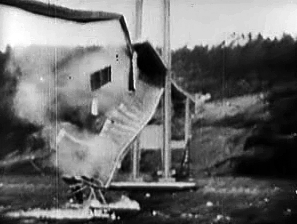
\includegraphics[width=0.75\textwidth]{../sections/seasons/season1/105/images/105a.png} 
	\end{figure}


Imagine a young child is sitting on a swing. As is usually the case in homework problems from physics textbooks, you find that attached to the child is a large spring. You stretch and relax the spring at various constant frequencies. As you vary the frequency of this stretching and relaxing, you notice that if the frequency is very high, the child doesn't swing very high. The same thing happens when you push and pull at very low frequency. As you increase the frequency from low to high, you notice that the child starts swinging higher and higher until at a certain frequency it peaks and then starts to fall down again.  The frequency in the middle is the maximum resonance frequency. The oscillatory behavior of the child swinging (a pendulum) and the oscillatory motion of you stretching and relaxing interact with one another. At low and high frequencies, they work against one another too much and the swing won't move very much. At that maximum resonance frequency, though, the oscillation of the rubber band is amplifying the motion of the swing as much as possible. 


The same phenomena is found throughout nature. The famed singing woman who can break a wine glass is theoretically possible. When sound is directed toward the glass, the bulb of the wine glass begins to stress and strain, though it looks like it is just shaking. If the sound is at the correct frequency (and of sufficient volume), then the strain from the oscillations will exceed the elasticity of the glass and shatter it. The same volume which shatters the glass will be completely useless at other frequencies.  In fact if the wind hits a poorly designed bridge just right, the bridge will begin to twist to the point where it tears itself apart. The problem Charlie is working on in this episode is to determine whether the wind blowing against the side of the building could cause enough strain to buckle the building. Obviously the wind is not strong enough to physically push the building over, but the with the fluid flow across the building, factors like resonance can be huge.


The general equation which governs fluid flow is called the Navier-Stokes equation. This equation is a non-linear partial differential equation. As a result, it exhibits chaotic behavior called turbulence. This means that even though two points are relatively close to one another in position, the forces at each of those two points could be vastly different. For example, in the eye of a hurricane, there is almost no wind at all, and yet just outside this small region, the winds are strong enough to tear the roof off a house.  When a plane takes off, the airflow immediately below the plane is powerful enough to throw a car, and yet the wheels of the plane are not destroyed. \bref{Chaos}{https://en.wikipedia.org/wiki/Chaos_theory} is a property which results from non-linearity: solutions to non-linear equations are extremely sensitive on initial conditions. This is one reason why the weather is so hard to predict. Simply approximating wind speed at a point is enough for the resulting weather patterns to be completely different from reality over a very short period of time. This is popularly called the Butterfly Effect - a butterfly flapping its wings in Brazil could be the difference between clear skies and tornados in Texas, to paraphrase the title of a talk given by the physicist Lorenz. The Navier-Stokes equation is so complicated that, despite being generally accepted as correct, no one has found a long-time solution to it. Anyone who can find such a solution (or prove none exists) will receive a \$1,000,000 prize from the Clay Institute.


Fluid flow is not just important in construction. Animal flight is even more complicated than airplanes since the wings can move in complicated ways. Why do large birds fly differently from small insects?  How does the bumblebee fly? Its flight was not well-understood until the last few years. This glaring inability to explain something so simple was one of the greatest failures of science. Its wing size and number of flaps per minute were not enough to explain how it could keep itself aloft. Its unique style of flight is something noticed long ago. In fact, in 1934 a french entomologist claimed that the flight of the bumblebee was aerodynamically impossible. However, in 2005 high speed digital photography was able to show how the wings of the bee flap. As mentioned in the episode, the way blood flows through the body is an important factor in forensic medicine, let alone medicine proper.